\documentclass{article}
\usepackage{graphicx}

\title{Persistent Data Structures\\ 6.854 Scribe Notes \#2}
\date{September 8, 2006}
\author{Lecturer: David Karger\\ Scribe: David Glasser}

\begin{document}

%%%%%%%%%%%%%%%%%%%%%%%%%%%%%%%%%%%%%%%%%%%%%%%%%%%%%%%%%%%%%%%%%%%%%%
% Lecture command takes 4 arguments:
%               ordinal number of the lecture
%               date of the lecure
%               lecturer
%               scribe---that is you.
%
% Fill out the next line with this information !!!!

%%%%%%%%%%%%%%%%%%%%%%%%%%%%%%%%%%%%%%%%%%%%%%%%%%%%%%%%%%%%%%%%%%%%%%
% Your notes start here!
%%%%%%%%%%%%%%%%%%%%%%%%%%%%%%%%%%%%%%%%%%%%%%%%%%%%%%%%%%%%%%%%%%%%%%
%
% For theorems, lemmas, definitions, remarks, etc. use commands
% {\theorem{...}}, {\lemma{...}}, {\definition{...}}, etc.
% For proofs, use \begin{proof} ... \end{proof}
%
% For postscript figures (.ps) use the following block:
%
% \begin{figure}[h]
% \begin{center}
% \mbox{\psfig{figure=notes-nn-fig-mm.ps}}
% \caption{A very nice picture.}
% \label{fig:picture}
% \end{center}
% \end{figure}
%

% For encapsulated postscript figures (.eps) use the following block:
%  (also change documentstyle line )
% \begin{figure}[h]
% \begin{center}
% \mbox{\epsfbox{notes-nn-fig-mm.eps}}
% \caption{A very nice picture.}
% \label{fig:picture}
% \end{center}
% \end{figure}
%

%%%%%%%%%%%%%%%%%%%%%%%%%%%%%%%%%%%%%%%%%%%%%%%%%%%%%%%%%%%%%%%%%%%%%%

\section{Introduction and motivation}
\label{crp}

So far, we've seen only ephemeral data structures.  Once changes have been made to an
ephemeral data structure, no mechanism exists to revert to  previous states.  Persistent
data structures are really data structures with archaeology.

Partial persistence lets you make modifications only to the present data structure but
allows queries of any previous version.  These previous versions might be accessed via
a timestamp.

Full persistence lets you make queries and modifications to all previous versions of the
data structure.  With this type of persistence the versions don't form a simple linear
path --- they form a version tree.

The obvious way to provide persistence is to make a copy of the data structure each time it is changed.

This has the drawback of requiring space and time proportional to
the space occupied by the original data structure.

It turns out that we can achieve persistence with $O(1)$ additional
space and $O(1)$ slowdown per operation for a broad class of data
structures.

\subsection{Applications}

In addition to the obvious ``look-back'' applications, we can use
persistent data structures to solve geometric problems by representing
one of their dimensions as time.

Once example is the computational geometry problem of planar point
location. Given a plane with various polygons or line segments which
break the area up into a number of regions, in which region is a query
point is located?

In one dimension, the linear point location problem can be solved with
a splay tree or a binary tree, or even just a sorted array, that
simply searches for the two objects on either side of the query point.
So in one dimension, this problem can be solved in $O(\log n)$ time.

\begin{figure}[ht]
\begin{center}
  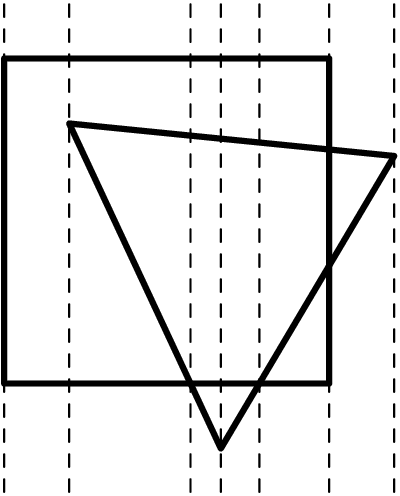
\includegraphics{scribe5fig.4.png}
\end{center}
\caption{Breaking the plane into slices for planar point location}
\label{fig:ppl}
\end{figure}

To solve the problem in two dimensions, break the plane into vertical
slices at each vertex or point where lines cross. These slices are
interesting because crossovers don't happen inside slices: inside each
slice, the dividing lines between regions appear in a fixed order, so
the problem reduces to the linear case and requires a binary search
(plus a bit of linear algebra).  Figure~\ref{fig:ppl} shows an example
of how these slices look. To locate a point, first find the vertical
slice it is in with a search on the point's x coordinate, and then,
within that slice, find the region it is in with a search on the
point's y coordinate (plus algebra). To do two binary searches takes
only $O(\log n)$ time, so we can locate a point in $ O(\log n)$ time.
However, setting up the trees for searching a figure with $n$ vertices
will require $n$ different trees, and each tree will take
$O(n\log n)$ time for sorting, so in total it takes $O(n^2 \log n)$ time and
$O(n^2)$ space to do the preprocessing.

Suppose that the points in the input are in general position -- that is 
no two have the same X or Y coordinate. Then between two adjacent slices
of the picture, there can be at most one segment being removed and at most
one segment being added. With points not in general position, we could either
randomly perturb the input or allow slices of width 0.
If we treat the horizontal direction as a timeline and
use a persistent data structure, we can find the horizontal location
of the point as a `version' of the vertical point location data
structure. So instead of thinking of the question as ``in what
two-dimensional region is the point $(x,y)$?'', we can think of it as
``at time $t$, in what one-dimensional region is the point $y$?''.
Every time we move to the next slab, we only have to insert or delete
at most one region from a single persistent binary search tree.  In
this way, as long as we can keep the tree balanced, we can preserve
the $O(\log n)$ query time and use only $O(n\log n)$ preprocessing
time and $O(n)$ space.



\section{Making pointer-based data structures persistent}

Now let's talk about how to make arbitrary pointer-based data structures
persistent. Eventually, we'll reveal a general way to do this with $O(1)$
additional space and $O(1)$ slowdown, first published by Sleator and Tarjan
et al. We're mainly going to discuss partial persistence to make the
explanation simpler, but their paper achieves full persistence as well.


\subsection{First try: fat nodes}

One natural way to make a data structure persistent is to add a
modification history to every node. Thus, each node knows what its value
was at any previous point in time. (For a fully persistent structure, each
node would hold a version tree, not just a version history.)

This simple technique requires $O(1)$ space for every modification: we just
need to store the new data. Likewise, each modification takes $O(1)$
additional time to store the modification at the end of the modification
history. (This is an amortized time bound, assuming we store the
modification history in a growable array. A fully persistent data structure
would add $O(\log m)$ time to every modification, since the version
history would have to be kept in a tree of some kind.)

Unfortunately, accesses have bad time behavior. We must find the right
version at each node as we traverse the structure, and this takes time. If
we've made $m$ modifications, then each access operation has $O(\log m)$
slowdown, and a query in our region computation will take $O(\log^2 n)$ time: not so great.
(In a partially persistent structure, a version is uniquely
identified by a timestamp. Since we've arranged the modifications by
increasing time, you can find the right version by binary search on the
modification history, using the timestamp as key. So it takes $O(\log m)$
time to find the last modification before an arbitrary timestamp. The time
bound is the same for a fully persistent structure, but a tree lookup is
required instead of a binary search.)


\subsection{Second try: path copying}

Another simple idea is to make a copy of any node before changing
it. Then you have to cascade the change back through the data
structure: all nodes that pointed to the old node must be modified
to point to the new node instead. These modifications cause more
cascading changes, and so on, until you reach a node that nobody
else points to---namely, the root. (The cascading changes will
always reach the root.) Maintain an array of roots indexed by
timestamp; the data structure pointed to by time $t$'s root is
exactly time $t$'s data structure. (Some care is required if the
structure can contain cycles, but it doesn't change any time
bounds.)  (Random note: this happens to be the data model for the
repository in the Subversion version control system.)

Figure~\ref{pathcopy} shows an example of path copying on a binary search
tree. Making a modification creates a new root, but we keep the old root
around for later use; it's shown in dark grey. Note that the old and new
trees share some structure (light grey nodes).

\begin{figure}[ht]
\begin{center}
  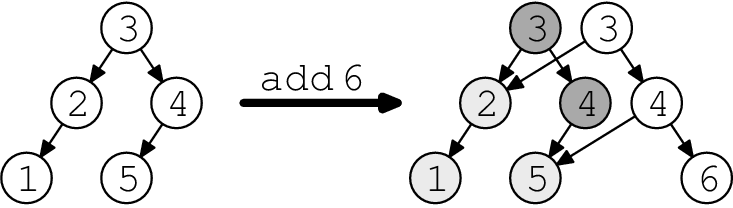
\includegraphics{scribe5fig.1.png}
\end{center}
\caption{Path copying on binary search trees}
\label{pathcopy}
\end{figure}

Access time does better on this data structure. Accesses are free, except
that you must find the correct root. With $m$ modifications, this costs
$O(\log m)$ additive lookup time---much better than fat nodes'
multiplicative $O(\log m)$ slowdown, and lets us keep the $O(\log n)$ query
time in our region application.

Unfortunately, modification time and space is much worse. In fact, it's
bounded by the size of the structure, since a single modification may cause
the entire structure to be copied. That's $O(m)$ for one update, and thus
$O(n^2)$ preprocessing time in the region application.

Path copying applies just as well to fully persistent data structures.


\subsection{Sleator, Tarjan et al.}

Sleator, Tarjan et al. came up with a way to combine the advantages of fat
nodes and path copying, getting $O(\log m)$ access time and $O(1)$
modification space and time. Here's how they did it, in the special case of
trees.

In each node, we store one \emph{modification box}. This box can hold one
modification to the node---either a modification to one of the pointers, or
to the node's key, or to some other piece of node-specific data---and a
timestamp for when that modification was applied. Initially, every node's
modification box is empty.
We can think of this as being a very short log with at most one entry.

Whenever we access a node, we check the modification box, and compare its
timestamp against the access time. (The access time specifies the version
of the data structure that we care about.) If the modification box is
empty, or the access time is \emph{before} the modification time, then we
ignore the modification box and just deal with the normal part of the node.
On the other hand, if the access time is \emph{after} the modification
time, then we use the value in the modification box, overriding that value
in the node. (Say the modification box has a new \texttt{left} pointer.
Then we'll use it instead of the normal \texttt{left} pointer, but we'll
still use the normal \texttt{right} pointer.)

Modifying a node works like this. (We assume that each modification touches
one pointer or similar field.) If the node's modification box is empty,
then we fill it with the modification. Otherwise, the modification box is
full. We make a copy of the node, but \emph{using only the latest values}.
(That is, we overwrite one of the node's fields with the value that was
stored in the modification box.) Then we perform the modification directly
on the new node, without using the modification box. (We overwrite one of
the new node's fields, and its modification box stays empty.) Finally, we
cascade this change to the node's parent, just like path copying. (This may
involve filling the parent's modification box, or making a copy of the
parent recursively. If the node has no parent---it's the root---we add the
new root to a sorted array of roots.)

Figure~\ref{slt-mod} shows how this works on a persistent search tree. The
modification boxes are shown in grey.

\begin{figure}[ht]
\begin{center}
  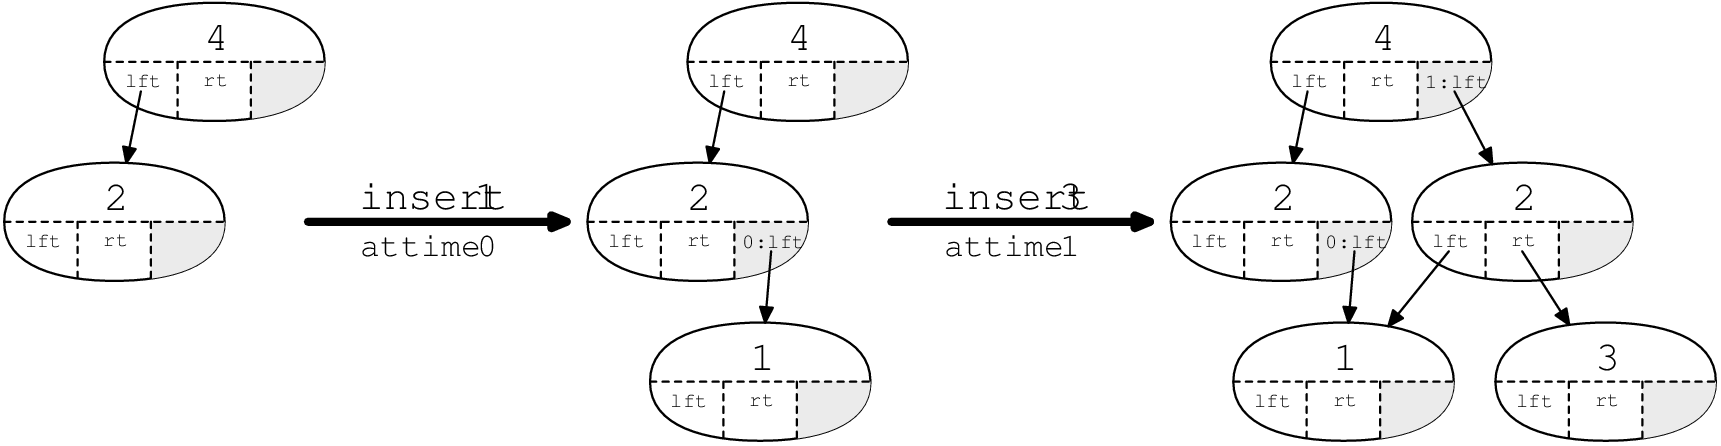
\includegraphics{scribe5fig.3.png}
\end{center}
\caption{Modifying a persistent search tree.}
\label{slt-mod}
\end{figure}

With this algorithm, given any time $t$, at most one modification box
exists in the data structure with time $t$. Thus, a modification at time
$t$ splits the tree into three parts: one part contains the data from
before time $t$, one part contains the data from after time $t$, and one
part was unaffected by the modification.

\begin{figure}[ht]
\begin{center}
  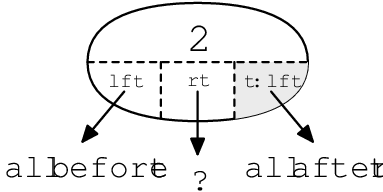
\includegraphics{scribe5fig.2.png}
\end{center}
\caption{How modifications split the tree on time.}
\label{split-time}
\end{figure}

How about time bounds? Well, access time gets an $O(1)$ slowdown (plus an
additive $O(\log m)$ cost for finding the correct root), just as we'd
hoped! (We must check the modification box on each node we access, but
that's it.)

Time and space for modifications require amortized analysis. A
modification takes $O(1)$ amortized space, and $O(1)$ amortized time.
To see why, use a potential function $\Phi$, where $\Phi(T)$ is
\emph{the number of full live nodes in $T$}.
(We can remember this as ``fat children have potential''.)
The live nodes of $T$ are
just the nodes that are reachable from the current root at the current
time (that is, after the last modification). The full live nodes are
the live nodes whose modification boxes are full.

So, how much does a modification cost? Each modification involves some
number of copies, say $k$, followed by 1 change to a modification box.
(Well, not quite---you could add a new root---but that doesn't change the
argument.) Consider each of the $k$ copies. Each costs $O(1)$ space and
time, but decreases the potential function by one! (Why? First, the node we
copy must be full and live, so it contributes to the potential function.
The potential function will only drop, however, if the old node isn't
reachable in the new tree. But we know it isn't reachable in the new
tree---the next step in the algorithm will be to modify the node's parent
to point at the copy! Finally, we know the copy's modification box is
empty. Thus, we've replaced a full live node with an empty live node, and
$\Phi$ goes down by one.) The final step fills a modification box, which
costs $O(1)$ time and increases $\Phi$ by one.

Putting it all together, the change in $\Phi$ is $\Delta\Phi = 1 -
k$. Thus, we've paid $O(k + \Delta\Phi) = O(1)$ space and $O(k +
\Delta\Phi + 1) = O(1)$ time!

What about non-tree data structures? Well, they may require more than one
modification box. The limiting factor is the \emph{in-degree} of a node:
how many other nodes can point at it. If the in-degree of a node is $k$,
then we must use $k$ extra modification boxes to get $O(1)$ space and time
cost.


\subsection{The geometric search problem}

Let's return to the geometric search problem discussed in
Section~\ref{crp}. We now know how to make a persistent tree; but what kind
of balanced tree should we use?

It turns out that this is one application where splay trees crash and
burn.  The reason is splaying.  Every rotation while we access a splay
tree is a modification, so we do $O(\log n)$ modifications (costing an
additional $O(\log n)$ space) per access---including reads!

A less sexy balanced tree, like a red-black tree, is a better choice.
Red-black trees keep themselves balanced with at most one rotation per
modification (and a bunch of fiddling with red/black bits). This looks
good---accesses are cheaper, and modifications cost $O(1)$---almost. The
``almost'' is because of red/black bit fiddling, which may affect a lot
more than one node on the tree. A fully persistent red-black tree would
need to keep the proper values for the red/black bits for every single
version of the tree (so that further modifications could be made). This
would mean that changing a red/black bit would count as a modification, and
would have a persistence-related cost. Luckily, in the geometric search
problem, we won't need to look at the red/black bits when doing lookup
on old versions of the tree: we only use them during the preprocessing when
building the tree, and we only ever care about their newest value.
So we don't do any logging on the red-black bits: we'll only log and copy
when we change actual pointers.
So only a constant number of \emph{logged} changes happen in each operation,
so we pay $O(1)$ persistence-related cost per modification.

\end{document}

%%% Local Variables: 
%%% mode: latex
%%% TeX-master: t
%%% End: 
